\documentclass{article}
\usepackage{multirow}
\usepackage{subcaption}
\usepackage[labelformat=parens,labelsep=quad,skip=3pt]{caption}
\usepackage{graphicx}
\usepackage{textcomp}
\usepackage[ruled,vlined]{algorithm2e}
\SetKw{KwBy}{by}

\title{SmallDepthMask: Large DataSet Generation for Monocular Depth Estimation and Foreground Segmentation from few Internet Images}
% tyhink of a better one word instead of SmallDepthMask
% MoDES : Monocular Depth Estimation and Segmentation - A Dataset of Stray Bovine Animals

\begin{document}

\maketitle

\begin{abstract}
Segmentation of desired object along with depth estimation is useful in various scenaroes like (give some examples here). 
Any deep learning workflow to segment the desired foreground object in a scene require significant training data.
The data generation process usually involve expensive hardware or significant manual involvement (give a few examples). 
This paper presents a novel way to utilize only a small number of readily available png images with transparency for the foreground object, and representative
background images from the internet and combine them to generate a huge dataset for deep learning
utilizing current state of the art monocular depth estimation techniques. Few example applications show the efficacy of the training data on detecting 
cattle on road for autonomous driving application, etc. etc. (mention some others if few more people join in). The baseline models generalize 
well to real scenarios.
% below is what we wrote previously

Stray Cattle are found everywhere on the Indian roads.
According to a survey, several thousand accidents happen on Indian roads each year 
involving stray animals\footnote{http://timesofindia.indiatimes.com/articleshow/70965326.cms}. 
This paper presents a custom dataset of Stray Animals for Monocular Depth Estimation and Segmentation (MODES) 
which can help in automatically identifying, counting and describing them with deep learning. 
The novelty of this dataset is, it is created from the existing depth models and tools without using any hardware devices. 
The size of the dataset is 4M records, and overall it contains 12M images. 
This paper also presents a baseline model as the starting point to develop more recognition algorithms.
The MoDES dataset is publicly availble at\footnote{https://www.kaggle.com/bsridevi/modes-dataset-of-stray-animals}.



Dataset creation. 

This work experimentally produces a dataset of size 4M records, where each record is a combination of 4 images from a very limited input. The input taken to generate this dataset are 100 background images and 100 foreground images.

How this dataset is unique and differs from the existing ones?  Firstly, It is a dedicated dataset for stray animals. and Secondly, the large
volume of data recorded: 40,00,000 tuples where each tuple is composed of a RGB image, a depth image, and a mask of the animal. 

limitation lacking ground truth

Depth and foreground prediction.


Keywords : Dataset, Depth image, mask, Depth prediction,
\end{abstract}

 

\section{Introduction}
Expand the abstract with appropriate references. We need references for:
1. Monocular Depth
2. Image segmentation
3. Deep learning requiring large datasets
4. Generating data sets is cumbersome
5. Ours is novel work that uses few images to generate huge dataset that generalizes well
%Above From Abhinav


A depth image is an image channel in which each pixel relates to a distance between the image plane and the corresponding object in the RGB image. 
The Monocular Depth Estimation is the task of estimating scene depth using a single image\cite{abuolaim2020defocus}. 
RGBD image is a combination of a RGB image and its corresponding depth image\cite{zhang2018deep}.
 Depth information is integral to many problems in
robotics, including mapping, localization and obstacle avoidance for terrestrial and aerial vehicles, autonomous navigation, and in computer vision,
 including augmented and virtual reality\cite{marchand2015pose}. RGBD datasets usually collected using depth sensors, monocular cameras, 
 LiDAR scanners which are expensive and data collection is a time consuming job. This paper proposes a technique to come up with a dataset 
 by using existing depth predictor, High Quality Monocular Depth Estimation via Transfer Learning. This paper introduces MoDES, 
 a custom dataset that contains millions of depth and forground images of stray animals created from few images by leveraging existing, 
 accurate models and tools. This is an RGB-DM dataset that pair images with depth and mask. The datasets which involve depth cannot be 
 created using crowd source annotation, instead they rely on 3D range sensors. MoDES is experimentally created with the help of existing 
 depth predictors and foreground creators.

/*if we can come up with limitations of existing rgbd datasets... then we can write This paper present the XYZ dataset 
in an effort to address the aforementioned limitations of exisitng RGBD datasets.*/

Figure \ref{fig:sampledatarecord} represents a few representative examples from MoDES dataset.

\begin{figure}[h!]
\centering
  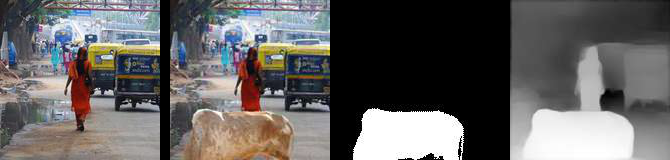
\includegraphics[width=1\textwidth]{samplerecord.png}
  \caption{Sample Record which contains the background image, a cow overlayed on top of background, its mask and depth images}
  \label{fig:sampledatarecord}
\end{figure}

The most important feature of MoDEs are -  It is an outcome of limited input. Every record in the dataset contains Background image, a background image on which a foreground image is overlay at random location, its respective mask, and dense depth image. Researchers can use this single dataset to do segmentation, train models to predict depth, or to predict both depth and mask. 

The main contributions of this paper are the following:
\begin{enumerate}
\item An approach to create larger datasets from the existing resources.
\item Building and releasing a custom dataset for Monocular Depth Estimation and Segmentation specific to stray animals.
\item Linking this dataset to a model.
\item The dataset and the trained models are publicly available.
\end{enumerate}

\begin{figure}[h!]
\centering
  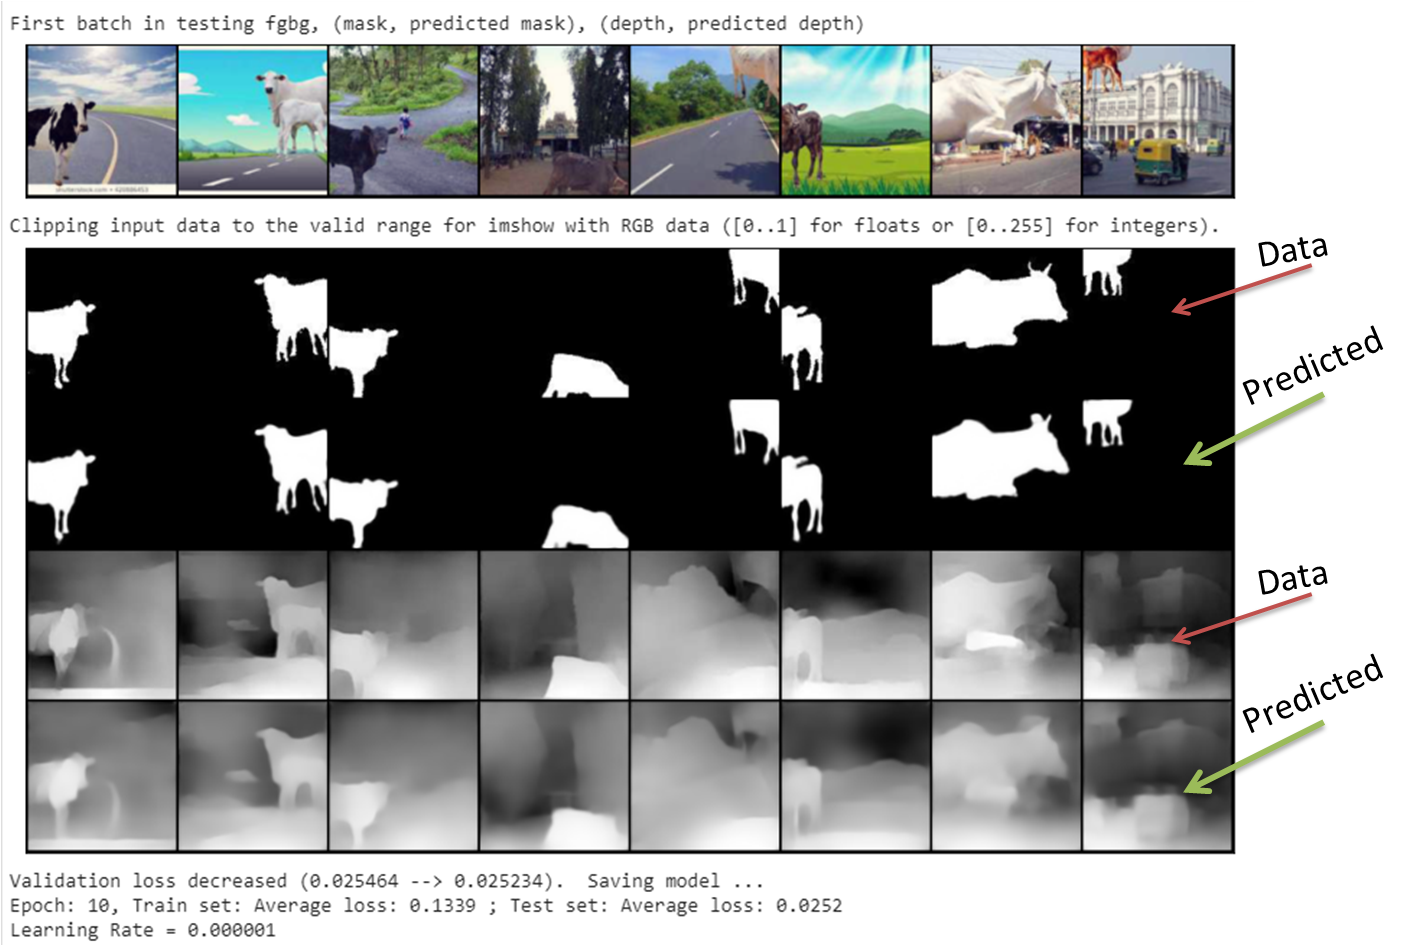
\includegraphics[width=1\textwidth]{finalepoch.png}
  \caption{Sample Record which contains the background image, a cow overlayed on top of background, its mask and depth images}
  \label{fig:samplerecord}
\end{figure}


\begin{figure}[h!]
\centering
  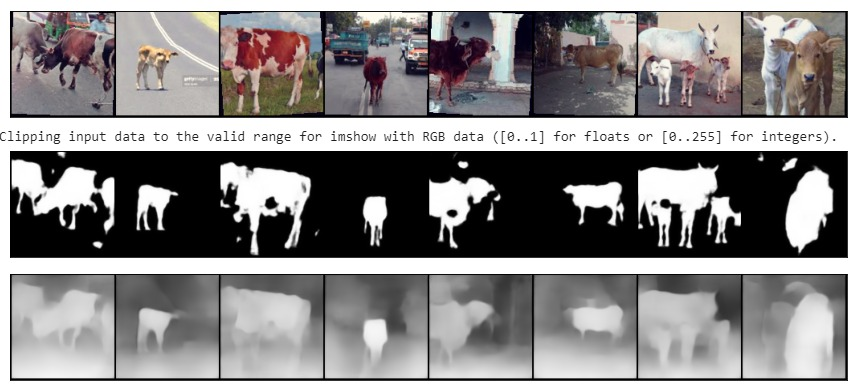
\includegraphics[width=1\textwidth]{unseen.jpeg}
  \caption{Sample Record which contains the background image, a cow overlayed on top of background, its mask and depth images}
  \label{fig:samplerecord}
\end{figure}


\section {Related Work}
We can include detailed study of related work here while in intro only mention few points with references. Same referencnes can be elaborated here. 
% Above from Abhinav
[*** sentences need to be reframed with the help of Abhinav sir
A variety of RGBD datasets in which images are paired with corresponding depth maps(D) have been proposed through the years.
Some of the RGBD datasets which are used mostly are kitti dataset~\cite{geiger2013vision}, the Synthia dataset~\cite{ros2016synthia}, 
Make3D dataset~\cite{saxena2008make3d}, NYU dataset~\cite{silberman2012indoor}

The dataset kiiti~\cite{geiger2013vision} is the best known RGBD dataset collected using a vehicle equipped with a sparse Velodyne VLP-64 LiDAR 
scanner and RGB cameras, and features street scenes in and around the German city of Karlsruhe. 
Primary application of this dataset involves perception tasks in the context of self-driving. 
Synthia~\cite{ros2016synthia} is a street scene dataset with depth maps of synthetic data, requiring domain adaptiation to apply to 
real world settings. Cityscapes~\cite{cordts2016cityscapes} provides a dataset of street scenes, albeit with more diversity than KITTI. 
Sintel~\cite{mayer2016large} is another synthetic dataset which mainly comprises of outdoors sences. 
Megadepth~\cite{li2018megadepth} is a large-scale dataset of outdoor images collected from internet, with depth maps reconstructed 
using structure-from-motion techniques, but this dataset lacks in ground truth depth and scale.
Make3D~\cite{saxena2008make3d} provides RGB and depth information for outdoor scenes. 
The NYUv2 dataset~\cite{silberman2012indoor} is widely used for monocular depth estimation in indoor environments. 
The data was collected with a Kinect RGBD camera, which provides sparse and noisy depth returns. 
These returns are generally in- painted and smoothed before they are used for monocular depth estimation tasks. 
As a result, while the dataset includes sufficient samples to train modern machine learning pipelines,
the “ground-truth” depth does not necessarily correspond to true scene depth.

Most of the existing datasets consists of indoor images, or outdoor images of city streets. 
There is no specific dataset which contains the animals which freely roam on roads without considering any traffic rules.
With an intention identify and recognize these animals, authors have come up with a dataset. 
Most of the datasets, except Megadepth were collected using cameras or sensors. 
Motivated from MegaDepth, our work curates a dataset of Animals, which are majority found on the roads, by using few cow, 
calf, buffalo images and few background images.
***]

\section{Dataset Generation Method}
we designed the dataset with the following objectives...
\begin{enumerate}
\item dataset which dedicatedly include foreground object. 
\item dataset should drive deep learning models and generalize. 
\item dataset should provide accurate dense depth maps.
\item dataset should provide foreground images
\end{enumerate}

\subsection{Data Acquisition}
The Related work says that the depth measurement took place with variety of devices like kinects, structure light cameras, and LiDAR etc. 
This work mainly focusing on the generation of huge dataset with limited availability of scene images and foreground images. 
This work generates foreground images and masks using GIMP~\cite{howat2014greenland} software and 
depth maps by using the model proposed by Ibraheem Alhashim et al. in their paper titled "High Quality Monocular Depth Estimation 
via Transfer Learning"~\cite{alhashim2018high} and the source code is available 
at \footnote{https://github.com/ialhashim/DenseDepth/blob/master/DenseDepth.ipynb}. 
The main source images for the dataset are 100 scene images, and 100 images of objects. 
We are referring scene images here as background images. 
They consists of the locations where stray animals usually move, like streets, main roads, front view of shops, markets, 
railway tracks, landscapes etc. A maximal random crop of $448 X 448$ without affecting the image aspect is done on 
background images. The object picked for this custom dataset creation is stray animals (mostly cows/bull/calf etc.). 
We have taken care to include single animals, group of animals, front, back and side poses of animals, 
all age group animals, and many coloured cows. 
Figure shows few of the sample background and foreground images used for the creation of this dataset. 
From these 100 selected foreground objects, we have created 200 transparent objects. 
Several tools like Photoshop's magic wand, lasso tool, 
online resources to remove backgrounds\footnote{https://www.remove.bg/}, 
were used to create transparent foreground images. These 100 images are flipped horizontally to get 200 
foreground images. Fig. \ref{fig:input-images} shows a sample set of background images and transparent foreground images.

\begin{figure}[h]
\centering
\begin{tabular}{c}
\subfloat[] {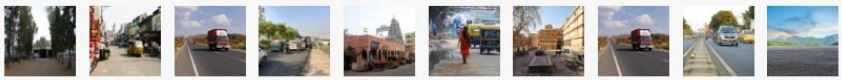
\includegraphics[scale=0.55]{bgimages.jpg}}
\end{tabular}
\begin{tabular}{c}
\subfloat[] {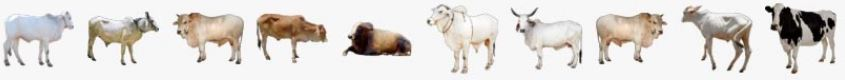
\includegraphics[scale=0.55]{fgimages.jpg}}
\end{tabular}

\caption{Some caption}
\label{input-images}
\end{figure}

\subsection{Data Curation and Processing}
To create the main dataset of 400K images, we used the selected 100 background images and the 200 foreground images. 
The entire procedure followed to create the dataset is represented in the form of algorithm. 

\begin{algorithm}[H]
\SetAlgoLined
\KwResult{creates 3 folders with fg\_bg, mask and depth each having 400K images} 
bg\_count := \textit{length(bg\_images list)} \;
fg\_count := \textit{length(fg\_images list)} \;

  \For{$i\gets1$ \KwTo $bg\_count$ \KwBy $1$}{
    \For{$i\gets1$ \KwTo $fg\_count$ \KwBy $1$}{
  \For{$i\gets1$ \KwTo $20$ \KwBy $1$}{
        randomly pick a center point (x, y)\;
     	randomly pick a scale \;
     	Place foreground on background by using scale and (x, y) \;
		calculate mask \;
    }
    }
	 \tcp*{Overlaying of all foreground images on a single background image is completed. }	    
    run depth model on 4K images\;
      }
\caption{Generate\_Dataset(\textit{[bgimages]}, \textit{[fgimages]})}
\end{algorithm}

\section{Example Applications}
\subsection{Detecting cattle on roads}
Describe importance and if possible related work and how deep learning is not yet applied.
Give example images


% From Abhinav
We can include adaptive placement of foreground to bemore realistic and also occlusion handling. However norte that this is only preliminary
The segmentation I used gave us road, skiy, tree etc. If I remember correctly, I used the bottommost row in image that have a threshold number of
sky pixels. And based on the max depth and span of the non sky part determined a formula to scale. The cattle was placed on ground area only
Finally, any objects that come on top of cow region in segmentation are put on top in the generated image.

I can formally write the algo tomorrow.
% end

\subsubsection{Baseline Model}
Discuss the model with loss function used and results along with generalized results

\subsection{Example 2} % if another partner comes

\subsection{Example 3} % for one more partner


\subsubsection{fg\_bg images}
To generate fg\_bg images, the foreground image is overlaid on background images randomly for 20 times. 
To place a foreground image on the background, a center point(x, y) in the range of 0 to 447 is randomly picked,
 and a scale between 0.3 to 0.6, which identifies the area overlaped by foreground image on the background image is also randomly picked. 
 Next the foreground image is scaled and placed on top of background image centered at (x, y). 
 Save this overlaid image with $224 \times 224$ resolution.   
 As the number of foreground images are 200, the total number of overlaid images per background becomes 4000. 
 By repeating the same procedure for all the 100 background images, the total number of fg on bg images becomes 400000. 
 A set of sample images after overlaying foreground on background are shown in Fig. 

\subsubsection{masks of fg\_bg images}
The mask is calculated for every fg\_bg image by setting a binary image to transparency channel of foreground image. 
These 400000 images are also stored in the particular folder of the dataset and a set of sample masks of fg on bg images are shown in Fig.  

\subsubsection{depth maps of fg\_bg images}
We used nyu.h5 model for depth calcualtion from Depth estimation proposed by~\cite{alhashim2018high}. 
This model requires input images to be of 448x448 resolution and produces 224x224 size depth image. 
A set of sample depth images are shown in fig.

\begin{figure}[h]
\centering
\begin{tabular}{c}
\subfloat[] {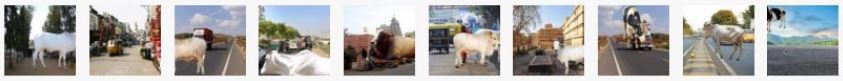
\includegraphics[scale=0.55]{overlay.jpg}}
\end{tabular}
\begin{tabular}{c}
\subfloat[] {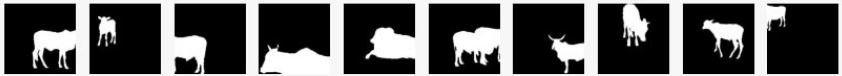
\includegraphics[scale=0.55]{overlaymask.jpg}}
\end{tabular}
\begin{tabular}{c}
\subfloat[] {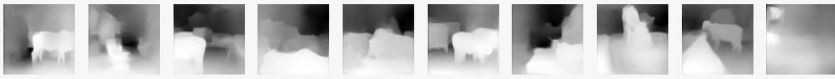
\includegraphics[scale=0.55]{overlaydepth.jpg}}
\end{tabular}

\caption{Some caption}
\label{MoDES dataset}
\end{figure}
\subsubsection{Directory Structure}


\subsection{Data Statistics}
Every image (fgbg, mask, depth) in the dataset are of size 224 X 224. 
The distribution of fgbg, mask and depth values for XYZ dataset are shown in fig. 
The dataset has 400000 records. A train-test-split of (70-30) gives a training set size of 280000 and 120000. 
A sample record in the dataset contains paths to all the images as shown below.

\textit{('./data/bgimages/bgimg099.jpg', 
'./data/out2/images/fgbg392483.jpg', 
'./data/out2/masks/mask392483.jpg', 
'./data/out2/depth/fgbg392483.jpg')}

\section{Experiments}
In this section, we provide a baseline for monocular depth estimation and segmentation on the XYZ dataset. 
The state-of-the-art models for image segmentation are variants of U-Net and fully convolutional networks (FCN)\cite{drozdzal2016importance}. 
long skip connections are used to skip features from the contracting path to the expanding path in order to recover 
spatial information lost during downsampling \cite{zhou2019unet++}. Short skip connections can be used to build deep FCNs. 
By using both long and short skip connections we proposed a model following U-Net architecture. 
This model has one encoder and two decoders, each meant for mask and depth prediction.
\subsection{Model}
We have designed a model with one encoder and two decoders with skip connections. 
The architecture is shown in Fig \ref{fig:modelarch}. The total no.of parameters of this model are 5,525,568. 
We have trained this model on the entire XYZ dataset from scratch. 
During training the network is trained with the batch size of 64 for 10 epochs using SGD optimizer \cite{bottou2010large}. 
We have used OneCycleLR scheduler \cite{smith2018disciplined} with a maximum Learning rate of 0.1. 
This made the initial learning rate as 0.0099.
The Deep Convolutional Neural Networks encoder is fed with a image (224 X 224) and the first decoder outputs a mask 
image and and second decoder outputs a depth image. To reduce overfitting\cite{perez2017effectiveness}, 
this work employed Random Rotation, Random Grayscale, Color Jitter, random horizontal flips and random chaneel swaps for data augmentation.

\begin{figure}[h!]
\centering
  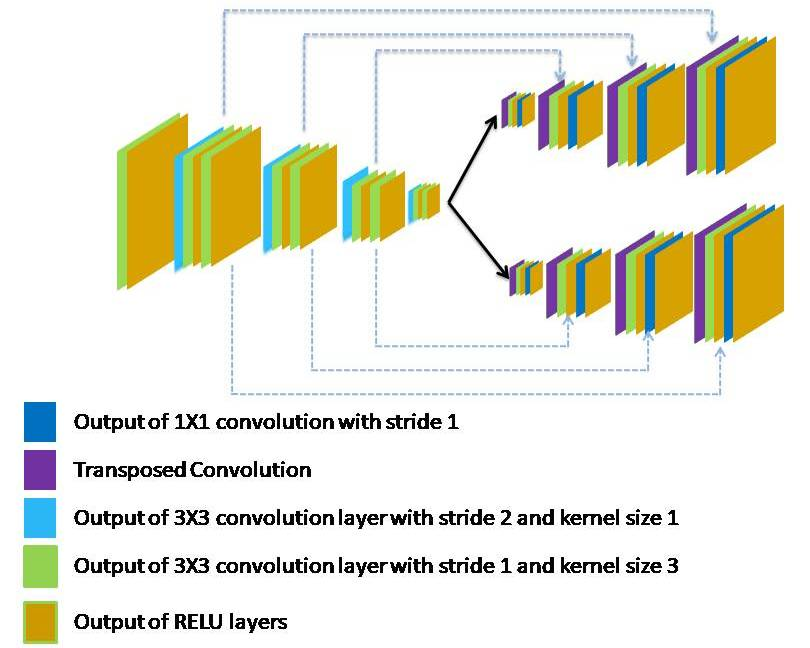
\includegraphics[width=1\textwidth]{networkarchitecture.jpg}
  \caption{Network Architecture}
  \label{fig:modelarch}
\end{figure}

The Loss is calculated with the help of L1 loss and Structural Similarity (SSIM) at both the decoders. 
We have also employed regularization for weight penality.

For training our network with two decoders, we defined the same loss function $L$ between $y$ and $\hat{y}$ as the weighted sum of 
two loss function values.

\begin{equation}
L(y, \hat{y}) = \lambda L_{term1}(y, \hat{y}) + (1 - \lambda) L_{term2}(y, \hat{y})
\end{equation}

The first loss term $L_{term1}(y, \hat{y})$ is the point-wise L1 loss defined on mask values at the first decoder and 
on depth values at the second decoder.

\begin{equation}
L_{term1}(y, \hat{y}) = \frac{1}{n} \sum_{x=1}^{n} \mid y_i - \hat{y_i} \mid
\end{equation}

we have also used weight decay... do we need to add it in the form of euation???????????

The second loss term $L_{term2}(y, \hat{y})$ uses a commonly used metric for image reconstruction task i.e., SSIM. 
Many recent tood depth prediction CNNs employed this metric. 
The loss term is redefined as shown in equation as SSIM has an upper bound of one.

\begin{equation}
L_{term1}(y, \hat{y}) = \frac{1 - SSIM(y, \hat{y})}{2}
\end{equation}

Different weight parameters $\lambda$ were tried and we have ended with a value $\lambda = 0.84$. The final loss function is as follows.

\begin{equation}
L(y, \hat{y}) = 0.84 \ast L_{term1}(y, \hat{y}) + 0.16 \ast L_{term2}(y, \hat{y})
\end{equation}

\subsection{Evaluation}
\subsection{Analysis}

3. 
\section{Conclusion}
\section{Acknowledgement}
This paper and the research behind it would not have been possible without the exceptional support and computing 
facilities of my Institution, Vishnu Institute of Technology. Ackowledge TSAI and Google Colab as well here.


\begin{thebibliography}{10}
\bibitem{abuolaim2020defocus} Abuolaim, Abdullah, and Michael S. Brown. "Defocus Deblurring Using Dual-Pixel Data." European Conference on Computer Vision. Springer, Cham, 2020.

\bibitem{zhang2018deep} Zhang, Yinda, and Thomas Funkhouser. "Deep depth completion of a single rgb-d image." Proceedings of the IEEE Conference on Computer Vision and Pattern Recognition. 2018.

\bibitem{geiger2013vision} Geiger, Andreas, et al. "Vision meets robotics: The kitti dataset." The International Journal of Robotics Research 32.11 (2013): 1231-1237.

\bibitem{ros2016synthia} Ros, German, et al. "The synthia dataset: A large collection of synthetic images for semantic segmentation of urban scenes." Proceedings of the IEEE conference on computer vision and pattern recognition. 2016.

\bibitem{cordts2016cityscapes} Cordts, Marius, et al. "The cityscapes dataset for semantic urban scene understanding." Proceedings of the IEEE conference on computer vision and pattern recognition. 2016.

\bibitem{mayer2016large} Mayer, Nikolaus, et al. "A large dataset to train convolutional networks for disparity, optical flow, and scene flow estimation." Proceedings of the IEEE conference on computer vision and pattern recognition. 2016.

\bibitem{saxena2008make3d} Saxena, Ashutosh, Min Sun, and Andrew Y. Ng. "Make3D: Depth Perception from a Single Still Image." AAAI. Vol. 3. 2008.

\bibitem{silberman2012indoor} Silberman, Nathan, et al. "Indoor segmentation and support inference from rgbd images." European conference on computer vision. Springer, Berlin, Heidelberg, 2012.

\bibitem{marchand2015pose} Marchand, Eric, Hideaki Uchiyama, and Fabien Spindler. "Pose estimation for augmented reality: a hands-on survey." IEEE transactions on visualization and computer graphics 22.12 (2015): 2633-2651.

\bibitem{alhashim2018high} Alhashim, Ibraheem, and Peter Wonka. "High quality monocular depth estimation via transfer learning." arXiv preprint arXiv:1812.11941 (2018).

\bibitem{li2018megadepth} Li, Zhengqi, and Noah Snavely. "Megadepth: Learning single-view depth prediction from internet photos." Proceedings of the IEEE Conference on Computer Vision and Pattern Recognition. 2018.

\bibitem{howat2014greenland} Howat, Ian M., A. Negrete, and Benjamin E. Smith. "The Greenland Ice Mapping Project (GIMP) land classification and surface elevation data sets." The Cryosphere 8.4 (2014): 1509-1518.

\bibitem{drozdzal2016importance} Drozdzal, Michal, et al. "The importance of skip connections in biomedical image segmentation." Deep Learning and Data Labeling for Medical Applications. Springer, Cham, 2016. 179-187.

\bibitem{zhou2019unet++} Zhou, Zongwei, et al. "Unet++: Redesigning skip connections to exploit multiscale features in image segmentation." IEEE transactions on medical imaging 39.6 (2019): 1856-1867.

\bibitem{bottou2010large} Bottou, Léon. "Large-scale machine learning with stochastic gradient descent." Proceedings of COMPSTAT'2010. Physica-Verlag HD, 2010. 177-186.

\bibitem{smith2018disciplined} Smith, Leslie N. "A disciplined approach to neural network hyper-parameters: Part 1--learning rate, batch size, momentum, and weight decay." arXiv preprint arXiv:1803.09820 (2018).

\bibitem{perez2017effectiveness} Perez, Luis, and Jason Wang. "The effectiveness of data augmentation in image classification using deep learning." arXiv preprint arXiv:1712.04621 (2017).

\end{thebibliography}
\end{document}
\section{Conclusion}
\section{Acknowledgement}
This paper and the research behind it would not have been possible without the exceptional support and computing facilities of my Institution, Vishnu Institute of Technology.
\begin{thebibliography}{10}



\end{thebibliography}
\end{document}==